\documentclass[a4paper]{article}

\usepackage[english]{babel}
\usepackage[utf8]{inputenc}
\usepackage{fullpage}
\usepackage{amsmath}
\usepackage{graphicx}
\usepackage[colorinlistoftodos]{todonotes}
%\usepackage{hyperref}
\usepackage{amssymb}
\usepackage{subfigure}
\usepackage{url}
\usepackage[pagebackref=true,colorlinks,linkcolor=red,citecolor=green,breaklinks=true,bookmarks=false]{hyperref}
\usepackage{outline} 
\usepackage{pmgraph} \usepackage[normalem]{ulem}
\usepackage{graphicx} \usepackage{verbatim}
\usepackage{indentfirst}
\usepackage{listings}
\usepackage{xcolor}
\setlength{\parindent}{2em}
% \usepackage{minted} % need `-shell-escape' argument for local compile

\title{
    \vspace*{1in}
    
\includegraphics[width=2.75in]{figures/zhenglab-logo} \\
    \vspace*{1.2in}
    \textbf{\huge Weekly Work Report}
    \vspace{0.2in}
}

\author{Hongzhi Liu \\
    \vspace*{0.5in} \\
    \textbf{VISION@OUC} \\
    \vspace*{1in}
}

\date{\today}


\begin{document}
\par
\maketitle
\setcounter{page}{0}
\thispagestyle{empty}

\newpage

\section{Research problem}

During this period of week, I spend time studying deep learning courses and working about Faster R-CNN algorithm for off-line test and FGFA algorithm for video object detection method in order to prepare URPC2018. Our team try to modify codes in project in order to output txt documents to evaluate algorithm performance. Besides, I download ILSVRC2015 DET and VID datasets to train a FGFA model and solve the problem in running code.

Because of difficulty in code modification, I have difficulty in adding codes to realize the function which can read test\_list.txt then output a txt which includes information about picture ID, class, confidence and correct bounding box. Furthermore, I need to rectify and debug the relevant codes of algorithm until they can meet the requirement to test and evaluate a contest model. At last, I should try to train a contest model by using flow guided feature aggregation algorithm. 

\section{Research approach}

In the process of research, I use the method of documentary analysis, comparative analysis and experimental research method. I read the thesis of Fast R-CNN \cite{Girshick2015Fast}, Faster R-CNN algorithm \cite{Ren2015Faster} and flow guided feature aggregation \cite{zhu17fgfa}. I try to unferstand core ideology in paper and learn about concept introduced by author.

Besides, I learn grammatical structure of python on the one hand, and on the other hand, I try to write script files to achieve batch processing commands. By this method, I can have a better understanding of python.

For deep learning, I watch the fourth course videos and write down the issues which I think are much important for further research. And then, I not only have learned the lessons of deep learning, but also put them into coding action. 


\section{Research progress}

During preparation for URPC2018, I receive two more kinds of image restoration datasets to train models and test how good the restoration algorithm are with mAP value. I continue to learn about Faster R-CNN algorithm \cite{Ren2015Faster} and relevant theory of flow guided feature aggregation \cite{zhu17fgfa}. Furthermore, I receive three datasets which have been image restored. By using the remote server, I try to train three knids of contest models with data sets and solve the porblem encounted when running a program with help of senior student. I will list details about weekly work in Tab.~\ref{t1} below. 

\begin{table}[hb]
	\centering
	\caption{Weekly work progress.}
	\begin{tabular}{c|p{10cm}}
		\hline 
		& Finish modifying codes in Faster R-CNN algorithm project.\\
		
		& Functions can be realized to read imformation in test\_list.txt and output the detection result.
		. \\
		
		URPC2018 &Finish test four image restoration method that are cla2, cla6, hsv and dcp and compare mAP value among them.\\
		
		& Succeed in running a demo of flow-guided feature aggregation for video object detection algorithm.\\
		\hline
		Deep Learning& Finish learning Convolutional Neural Networks which is the fourth course of deep learning.\\
		\hline
	\end{tabular}
	\label{t1}
\end{table} 


\section{Progress in this week}

During preparation for URPC2018, I have reordered four image restoration datasets upload to server. Then I spend time checking why output results of mAP value is too low and know the reason finally. After getting the correct result of mAP value of four image restoration methods, we compare them with origin picture to sum up experience. Besides, I modified code to make the output text is in correct method according to the official description. Furthermore, I can  run a FGFA demo and solve the problem in running code.  
\begin{description}
	\item [Step 1] Finish uploading cla2, cla6, hsv datasets which are reordered.
	\item[Step 2] Finish analyzing the low test value of output text and modifying codes in Faster R-CNN algorithm project.
	\item[Step 3] Finish outputting the correct txt to meet the requirement of contest and compare the method of image restoration.
	\item[Step 4] Finish learning Convolutional Neural Networks which is the fourth lesson.\label{t2}
\end{description}

\subsection{Data Sets}

In this week, our team product two new image restoration datasets that are dcp and dcp\_guided mothods as shown in Fig.~\ref{p1}. We train the contest model with the two datasets. Besides, I reordered cla2, cla6 and hsv pictures with thousands of image to train and test. Fig.~\ref{p1}\subref{p1a} is the picture restored by dcp method, Fig.~\ref{p1}\subref{p1b} is the picture restored by dcp\_guided method. And we use Algorithm~\ref{g1} to reorder name to VOC format.
\begin{figure}
	\centering 
	\subfigure[]{ 
		\label{p1a} %% label for first subfigure 
		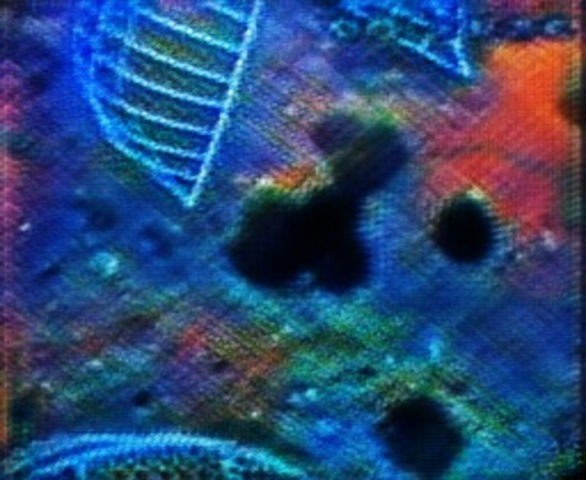
\includegraphics[width=7cm]{figures/1.jpg} 
	} 
	\subfigure[]{ 
		\label{p1b} %% label for second subfigure 
		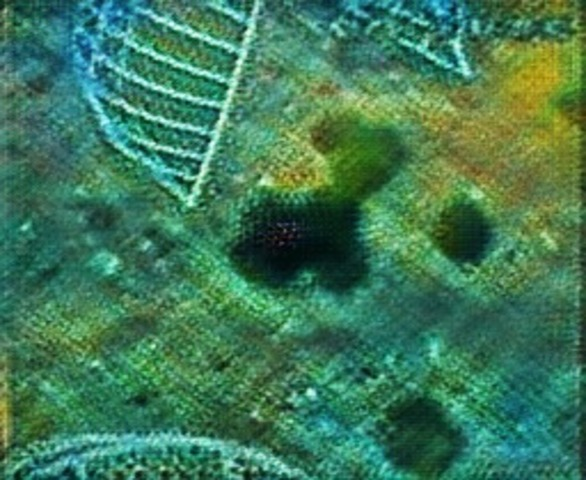
\includegraphics[width=7cm]{figures/2.jpg} 
	} 
	\caption{Two kinds of image restoration.} 
	\label{p1} %% label for entire figure 
\end{figure}

\lstset{language=python}
\begin{lstlisting}
import os
path = "/home/henry/File/URPC2018/VOC/VOC2007/JPEG/test/dcp"
path1 = "/home/henry/File/URPC2018/VOC/VOC2007/JPEG/test/train"
filelist = os.listdir(path)
for file in filelist: 
Olddir=os.path.join(path,file)  
if os.path.isdir(Olddir):   
continue
filename=os.path.splitext(file)[0]   
filetype=os.path.splitext(file)[1] 
Newdir=os.path.join(path1,str(int(filename)+1).zfill(6)+filetype) 
os.rename(Olddir,Newdir)
\end{lstlisting}\label{g1}


\begin{figure}
	\begin{center}
		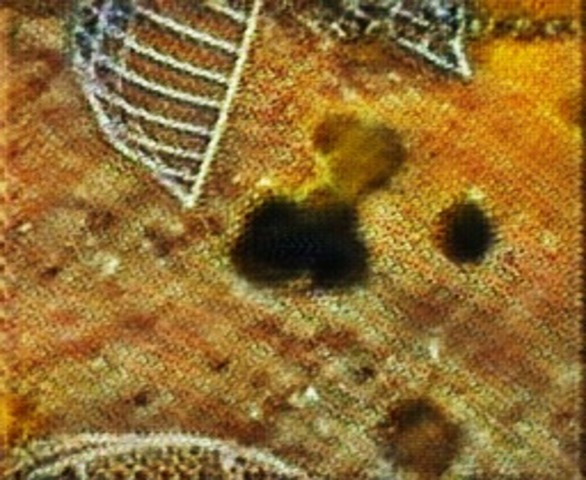
\includegraphics[scale=0.8]{figures/3.jpg}
	\end{center}
	\caption{Output results of several methods.}
	\label{p2}
\end{figure}

\subsection{Test a Contest Model}

When we first test model by using testlist.txt according to contest, we get a low value. After two days analysis, we know that we have wrong with ID and picture name. Then I try to modified codes in the project of Faster R-CNN files, relevant codes in pascal\_voc.py need to revise just as shown in Algorithm~\ref{g2}. At last, we successfully solved the problem. The results of methods can be seen in Fig.~\ref{p2}.


Furthermore, I should comparecheck total loss of my model to learn more about my model. Simulation results prove that this improved algorithm achieves an effect in accelerating the converging rate.

\begin{figure}
	\centering 
	\subfigure[]{ 
		\label{p3a} %% label for first subfigure 
		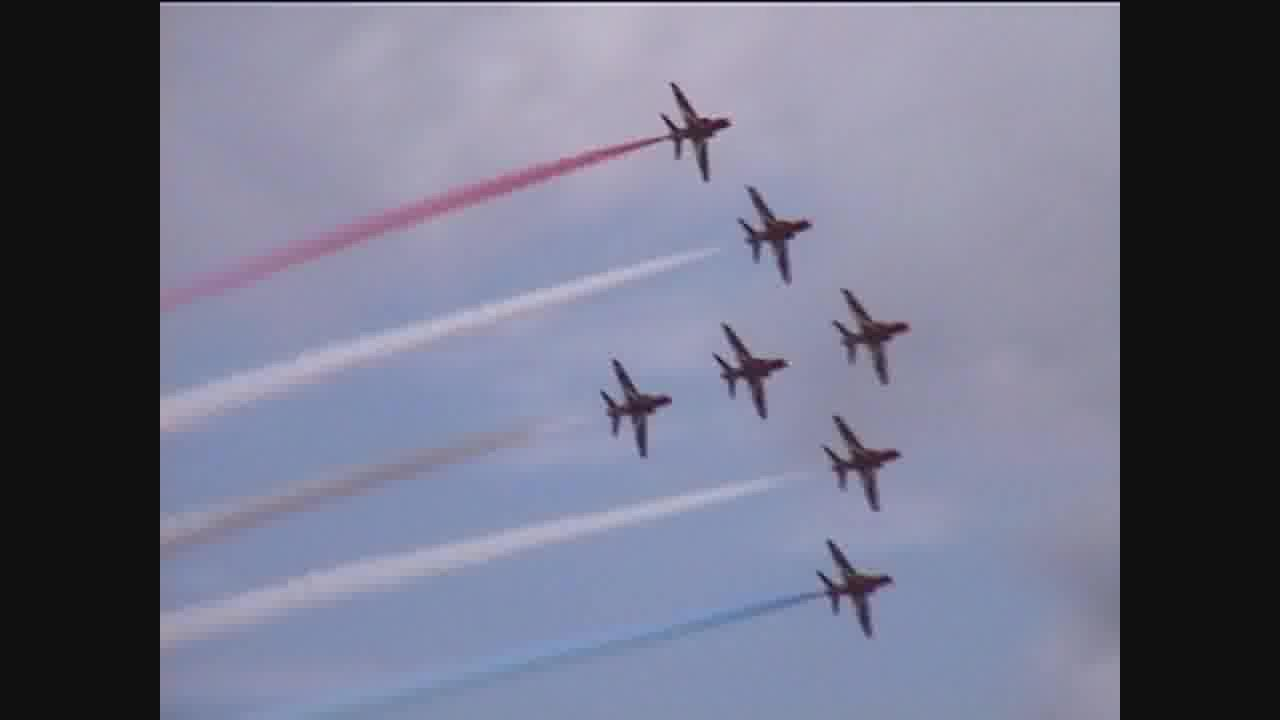
\includegraphics[width=6cm]{figures/5.JPEG} 
	} 
	\subfigure[]{ 
		\label{p3b} %% label for second subfigure 
		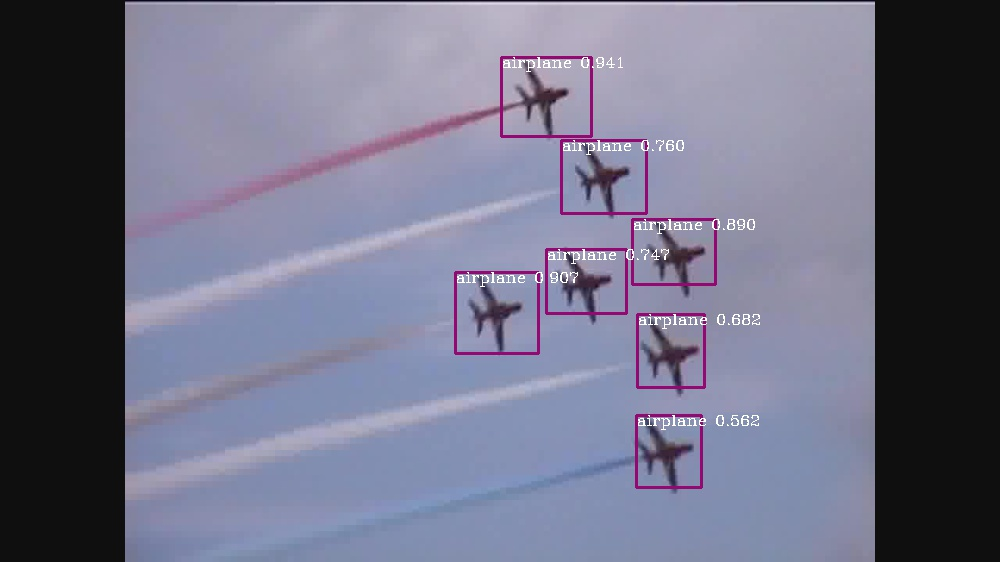
\includegraphics[width=6cm]{figures/4.JPEG} 
	} 
	\subfigure[]{ 
		\label{p3c} %% label for first subfigure 
		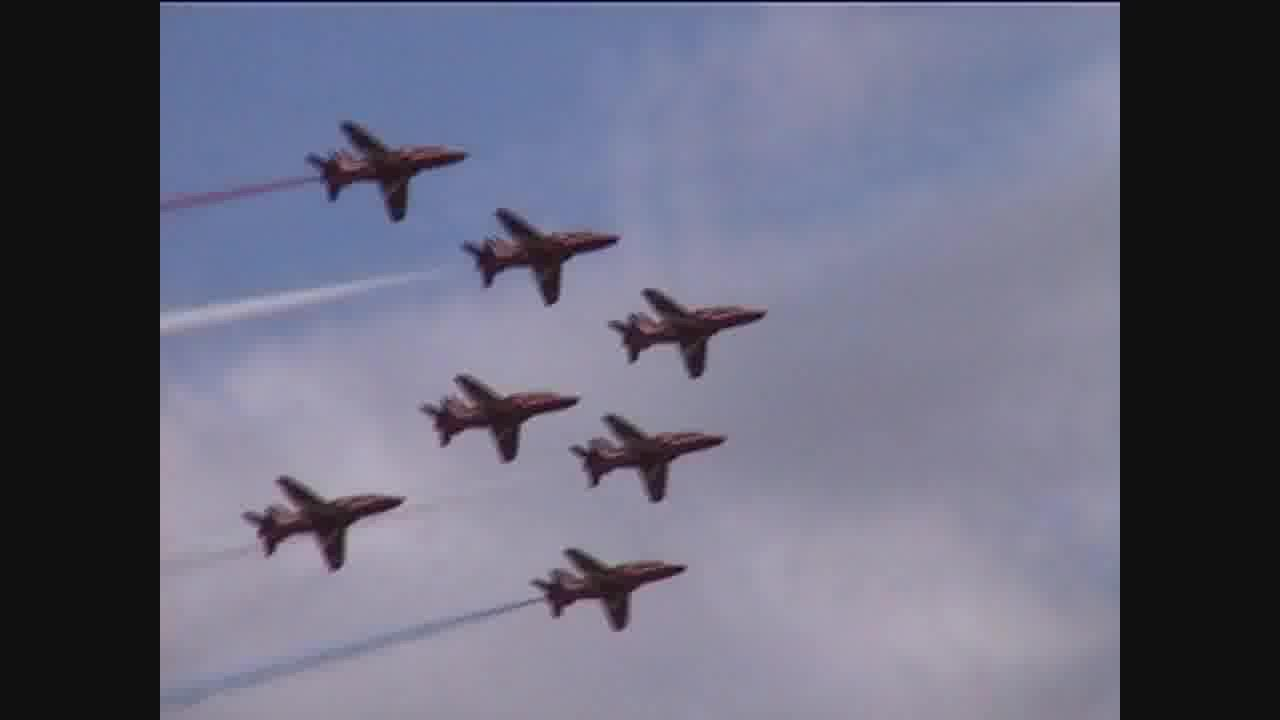
\includegraphics[width=6cm]{figures/7.JPEG} 
	} 
	\subfigure[]{ 
		\label{p3d} %% label for second subfigure 
		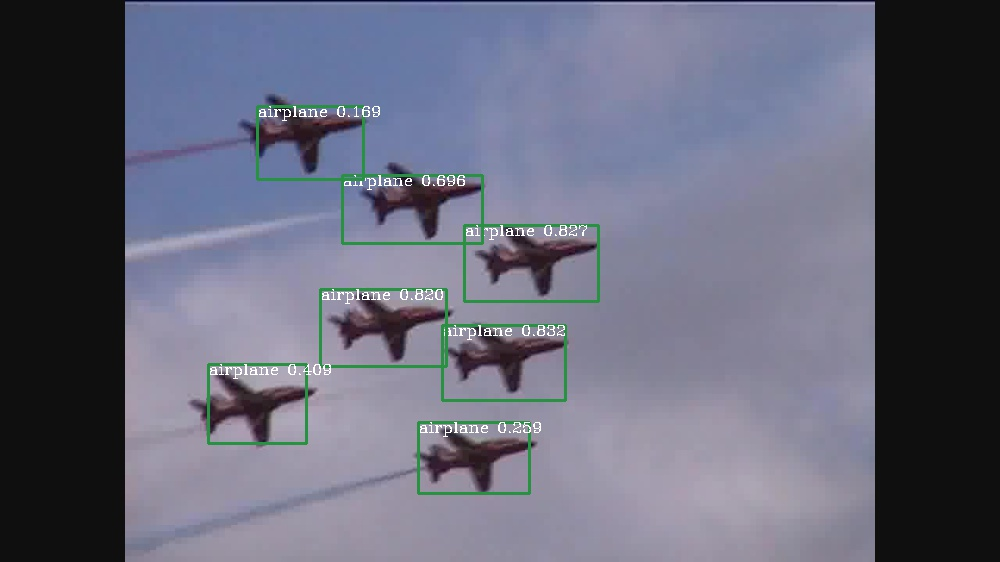
\includegraphics[width=6cm]{figures/6.JPEG} 
	} 
	\caption{Demo of flow-guided feature aggregation for video object detection.} 
	\label{p3} %% label for entire figure 
\end{figure}

\lstset{language=python}
\begin{lstlisting}
def demo(sess, net, image_name):
# Load the demo image
print('demoDemo for data/demo/{}{}'.format(im_name[0], '.jpg'))
print('demoDemo for data/demo/{}{}'.format(im_name[1], '.jpg'))
print('\n')

all_name = image_name+'.jpg'
im_file = os.path.join(cfg.DATA_DIR, 'demo', all_name)
im = cv2.imread(im_file)

fr = open('/home/henry/Files/tf-faster-rcnn-contest/data/VOCdevkit2007/test.txt', 'r')
for im_name in fr:
im_name = im_name.strip()
im_name = im_name.split(' ')
print('~~~~~~~~~~~~~~~~~~~~~~~~~~~~~~~~~~~')
print('mainDemo for data/demo/{}{}'.format(im_name[0],'.jpg'))
print('mainDemo for data/demo/{}{}'.format(im_name[1],'.jpg'))
print('\n')
demo(sess, net, im_name[0])
\end{lstlisting}\label{g2}

\subsection{Demo of FGFA}

There are some difficulties running the demo for us because of little issue reference in the github and blogs. So senior student and I try our best to solve the problems. And I can run a demo with somes picture just as shown in Fig.~\ref{p3}.

\section{Plan}

\begin{tabular}{rl}
	\textbf{Objective:} & Finish training a model with flow-guided feature aggregation for video object detection. \\
	\textbf{Deadline:} & 2018.08.15
\end{tabular}

\begin{description}
	\item[\normalfont 2018.07.16---2018.07.22] Finish neural networks and Deep Learning.
	\item[\normalfont 2018.07.23---2018.07.29] Finish improving deep neural networks courses.
	\item[\normalfont 2018.07.30---2018.08.05] Finish structuring machine learning projects courses.
	\item[\normalfont 2018.08.06---2018.08.12] Finish convolutional neural networks courses.
	\item[\normalfont 2018.08.13---2018.08.19] Finish sequence models courses.
\end{description}



% If you don't cite any references, please comment the following two lines
\bibliographystyle{ieee}
\bibliography{ref.bib}

\end{document}